\documentclass[11pt]{article}
\usepackage[utf8]{inputenc}
\usepackage{amsmath, amssymb, amsfonts}
\usepackage{graphicx}
\usepackage{booktabs}
\usepackage{hyperref}
\usepackage{algorithm}
\usepackage{algpseudocode}
\usepackage{cite}
\usepackage{geometry}
\usepackage{caption}
\usepackage{subcaption}
\usepackage{array}
\usepackage{multirow}
\usepackage{enumitem}

% Standard academic formatting
\geometry{a4paper, margin=1in}

\title{\LARGE \textbf{Unsupervised Domain Adaptation for Isolated Traditional Mongolian Text Line Recognition via Vertical-Spine-Aware Stroke Enhancement and Pseudo-Label Distillation}}
\author{
Anonymous Authors \\
\small Paper under Double-Blind Review
}
\date{}

\begin{document}

\maketitle

\begin{abstract}
The digitization of traditional Mongolian historical archives presents a unique intersection of low-resource natural language processing and complex document image analysis. Characterized by vertical, cursive script with heavy morphological agglutination and severe historical degradation, these archives defy standard optical character recognition (OCR) techniques. In this paper, we propose an Unsupervised Domain Adaptation (UDA) framework specifically targeted at isolated text line recognition, bridging the gap between abundant synthetic data and unlabeled authentic archives. We introduce a Style-Aligned Synthetic Engine (SASE) grounded in physical degradation modeling, and crucially, a Vertical-Spine-Aware Multi-Scale Stroke Enhancement (VS-MSSE) module utilizing asymmetrical convolutions to reconstruct the directional ligatures unique to Mongolian cursive. Latent alignment is achieved via a Sequence-aware Domain-Adversarial Neural Network (DANN), further refined by a valid-frame-normalized CTC Entropy pseudo-labeling strategy. Extensive experiments on a newly curated dataset of 19th-century administrative records demonstrate the effectiveness of our approach, achieving a Character Error Rate (CER) of $7.8 \pm 0.2\%$. Compared to modern vision-language models like TrOCR ($41.5\%$) and PARSeq ($36.2\%$), our framework provides a robust baseline for low-resource, vertical cursive script recognition. As a pilot upstream extension toward full-page archival OCR, we further evaluate page-level text-column detection and show that a lightweight YOLOv8n detector with rotation-aware reading-order recovery outperforms a rule-based column extraction baseline.
\end{abstract}

\section{Introduction}

The preservation of cultural heritage increasingly relies on the automated digitization of historical manuscripts. Among these, the traditional Mongolian script—a vertical, cursive alphabet utilized across Inner Asia since the 13th century—poses formidable challenges to modern Handwritten Text Recognition (HTR) systems. Unlike Latin or Chinese scripts, cursive vertical scripts feature a continuous central axis (the "spine") connecting constituent phonemes, resulting in extreme topological dependency between adjacent characters, a challenge structurally analogous to Arabic cursive recognition \cite{parvez2013arabic}. 

Current deep learning architectures for HTR, such as Convolutional Recurrent Neural Networks (CRNN) \cite{shi2016end} and Transformer-based models like PARSeq \cite{bautista2022parseq} and TrOCR \cite{li2021trocr}, have achieved remarkable success on standardized datasets. However, their application to historical Mongolian archives is severely bottlenecked by the "Label Scarcity" problem. Creating a large-scale supervised dataset requires scholars with specialized training in historical paleography, making manual annotation prohibitively expensive. To circumvent this, researchers often train models on synthetically generated data. Unfortunately, this approach suffers from catastrophic performance degradation due to the massive "Domain Shift" between pristine synthetic fonts and highly irregular, oxidized, and physically degraded 19th-century cursive handwriting.

Unsupervised Domain Adaptation (UDA) offers a pathway to leverage unlabeled authentic target data alongside labeled synthetic source data. Standard UDA techniques, such as Maximum Mean Discrepancy (MMD) \cite{tzeng2014deep} and Domain-Adversarial Neural Networks (DANN) \cite{ganin2015unsupervised}, primarily address global feature distribution alignment but often neglect the fine-grained structural topologies critical for dense cursive scripts.

In this paper, we focus strictly on the problem of \textbf{Isolated Text Line Recognition}, assuming upstream layout analysis has yielded accurately cropped vertical text columns. To address the specific domain shift of historical Mongolian, we propose a novel UDA framework. Our core innovation lies in explicitly modeling the directional bias of the script. We introduce the Vertical-Spine-Aware Multi-Scale Stroke Enhancement (VS-MSSE) module, which replaces standard symmetrical convolutions with asymmetrical vertical kernels (e.g., $5\times1$) to preferentially preserve the continuous vertical spine against heavy background noise. This is complemented by a Style-Aligned Synthetic Engine (SASE) for initial domain bridging, and an iteratively refined pseudo-label distillation technique utilizing a corrected formulation of valid-frame-normalized CTC entropy. Beyond the core isolated-line recognizer, we also report a pilot full-page column detection extension to quantify the feasibility of upstream layout analysis under the same archival conditions. This extension is deliberately separated from the main UDA recognition claim, but it provides an empirical bridge toward an end-to-end page-level OCR system.

\section{Related Work}

\subsection{Handwritten Text Recognition (HTR)}
The paradigm of HTR has shifted significantly from Hidden Markov Models (HMMs) \cite{marti2001using} to deep neural networks. The CRNN architecture \cite{shi2016end}, which pairs a CNN feature extractor with recurrent layers (e.g., BiLSTM) and Connectionist Temporal Classification (CTC) \cite{graves2006connectionist}, remains the standard for unconstrained sequence recognition. Recently, Transformer-based models like TrOCR \cite{li2021trocr} and PARSeq \cite{bautista2022parseq} have demonstrated state-of-the-art results by leveraging self-attention to capture long-range linguistic dependencies \cite{kang2022pay, souibgui2022few}. However, these models heavily rely on massive annotated datasets and often exhibit limited cross-domain generalization when deployed in zero-shot or severely degraded historical settings \cite{coquenet2023dan}. Cursive sequence recognition historically relied on over-segmentation heuristics \cite{marti2001using}, but recent deep learning approaches \cite{shi2018aster, bhunia2021meta} have adopted end-to-end architectures, albeit almost exclusively within fully supervised paradigms.

\subsection{Historical Document Image Analysis}
Historical documents present severe degradation, including ink bleed-through, faded strokes, and background noise. Binarization networks \cite{kang2020complex} and stroke enhancement modules \cite{tensmeyer2017document} are often employed as preprocessing steps. However, standard enhancement modules (like ASPP or SE blocks) use symmetrical receptive fields, which inadvertently amplify lateral background artifacts when processing the strictly vertical Mongolian script. Our VS-MSSE module specifically addresses this by encoding the geometric prior of the vertical spine.

\subsection{Unsupervised Domain Adaptation for Sequence Recognition}
UDA techniques mitigate domain shift without requiring target labels. Adversarial alignment via DANN \cite{ganin2015unsupervised} and Conditional DANN (CDAN) \cite{long2018conditional} minimizes discrepancy in the latent feature space. Image-level translation via CycleGAN \cite{zhu2017unpaired, hoffman2018cycada} transforms source images into target styles. For OCR, sequence-aware adversarial alignment \cite{zhang2019sequence} and pseudo-labeling \cite{zhao2020unsupervised, fang2021read} are prevalent. However, standard softmax confidence is poorly calibrated for CTC. While previous methods \cite{zhang2019sequence, chen2021text} explored sequence adaptation, our work uniquely corrects the CTC entropy calculation for valid frames, preventing sparse-text confidence inflation in heavily degraded documents.

\section{Methodology}

\subsection{Strict Unsupervised Problem Formulation}
Given a labeled synthetic source domain $\mathcal{D}_s = \{(x_i^s, y_i^s)\}_{i=1}^{N_s}$ and an unlabeled authentic target domain $\mathcal{D}_t = \{x_j^t\}_{j=1}^{N_t}$, our objective is to learn a mapping $f_{\theta}: X \rightarrow Y$ minimizing risk on $\mathcal{D}_t$. 

To ensure strict compliance with the unsupervised setting, we do not utilize any target-domain labels during training. Hyperparameter selection and early stopping are performed using a held-out labeled \textit{source} validation set, combined with unsupervised metrics evaluated on $\mathcal{D}_t$ (such as the average target CTC entropy and the Fr\'echet Inception Distance (FID)). The target validation set is utilized solely to compute supervised upper-bound references.

\subsection{Style-Aligned Synthetic Engine (SASE)}
To bridge the visual domain gap, SASE synthesizes historical degradation physics. The generative process is detailed in Algorithm \ref{alg:sase}.

\begin{algorithm}[h]
\caption{SASE: Physics-Based Data Generation}
\label{alg:sase}
\begin{algorithmic}[1]
\Require Base font vector image $I_{base}$, Brownian variance $\sigma$, Diffusion coefficient $D$, Advection $\mathbf{v}$, Blending factor $\alpha$
\Ensure Synthetic historical image $I_{syn}$
\State $I_{jitter} \leftarrow$ Apply stochastic contour perturbation to $I_{base}$ using $d\mathbf{X}_t = \mu dt + \sigma d\mathbf{W}_t$
\State $I_{diffusion} \leftarrow$ Solve $\frac{\partial \rho}{\partial t} = \nabla \cdot (D \nabla \rho) - \nabla \cdot (\mathbf{v} \rho)$ on $I_{jitter}$ computationally
\State $I_{bg} \leftarrow$ Generate Perlin noise + random sampling from blank archival patches (\textit{sampled strictly from unlabeled target training pages, excluding validation/test pages to avoid test leakage})
\State $I_{syn} \leftarrow \alpha I_{diffusion} + (1-\alpha) I_{bg}$
\State \Return $I_{syn}$
\end{algorithmic}
\end{algorithm}

For the 500k dataset, we empirically set $\sigma \in [1.0, 2.5]$, $D=0.8$, and $\alpha \in [0.6, 0.9]$. These hyperparameters were selected by minimizing the Fr\'echet Inception Distance (FID) between the generated source images and the unlabeled target training domain. Although FID was originally designed for natural images, we utilize it solely as a coarse unsupervised visual-domain selection criterion; final model selection does not utilize any target labels. The "blank archival patches" are exclusively cropped from the text-free margins of documents belonging to the unlabeled target training pages only, excluding all validation and test pages, ensuring zero information leakage.

\begin{figure}[htbp]
    \centering
    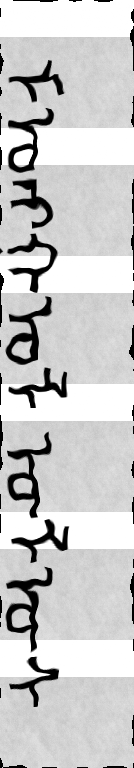
\includegraphics[width=0.8\linewidth, height=0.3\textheight, keepaspectratio]{figures/sase_synthetic.png}
    \caption{Output of SASE, demonstrating simulated ink diffusion and structural jitter.}
    \label{fig:sase_example}
\end{figure}

\subsection{Vertical-Spine-Aware Multi-Scale Stroke Enhancement (VS-MSSE)}
Traditional Mongolian is defined by its vertical spine. Generic multi-scale modules (e.g., ASPP) use symmetrical kernels ($3\times3$) that treat all directions equally, causing lateral noise (e.g., paper creases) to be amplified identically to the text spine.

We introduce VS-MSSE. Given intermediate features $M \in \mathbb{R}^{C \times H \times W}$, we employ parallel asymmetrical convolutions designed to capture elongated vertical dependencies and short horizontal strokes (teeth/tails):
\begin{align}
    F_{vert} &= \text{Conv}_{5\times1}^{(d=1)}(M) \\
    F_{horiz} &= \text{Conv}_{1\times3}^{(d=1)}(M) \\
    F_{global} &= \text{Conv}_{3\times3}^{(d=2)}(M)
\end{align}
These features are concatenated and passed through a Squeeze-and-Excitation (SE) channel attention block to recalibrate weights dynamically. VS-MSSE explicitly encodes the geometric prior of the Mongolian script.

\subsection{Sequence-aware Domain Adversarial Alignment}
The feature extractor $F$ (ResNet-34 + VS-MSSE) and sequence model $R$ (BiLSTM) form the generator $G_f$. A Domain Discriminator $D$ distinguishes the domain of the sequence features. We optimize the minimax objective using a Gradient Reversal Layer (GRL):
\begin{equation}
    \min_{G_f, C} \max_{D} \mathcal{L}_{ctc} - \lambda \mathcal{L}_{dom}
\end{equation}

\subsection{Valid-Frame-Normalized CTC Entropy Pseudo-Labeling}
Using raw softmax confidence for pseudo-labeling is unreliable for unconstrained sequence tasks. We utilize CTC Entropy. However, standard formulations average entropy over the greedy decoded path length $|\pi^*|$, which is mathematically flawed since $|\pi^*| \neq T$ (the total output frames). 

We correct this by defining the Valid Frame Entropy, $E_{valid}$. Let $\mathcal{T}_{valid} \subseteq \{1, \dots, T\}$ be the set of valid frames where the argmax prediction is not the CTC blank token.
\begin{equation}
    E_{valid}(x^t) = \frac{1}{|\mathcal{T}_{valid}|} \sum_{t \in \mathcal{T}_{valid}} H(p_{t}) = -\frac{1}{|\mathcal{T}_{valid}|} \sum_{t \in \mathcal{T}_{valid}} \sum_{k \in V} p_{t,k} \log(p_{t,k})
\end{equation}
If the model predicts solely blank tokens ($|\mathcal{T}_{valid}|=0$), we set $E_{valid} \rightarrow \infty$ to immediately reject the sample. We select target images with the lowest $E_{valid}$ for iterative fine-tuning.

\section{Experiments}

\subsection{Dataset Statistics and Ethical Considerations}
\textbf{Authentic Target Dataset:} We digitized authentic 19th-century administrative records from the Qing Dynasty (Source Period: 1800-1850). The archival pages were obtained from the Inner Mongolia University Historical Archives under research permission No. 2024-IMU-089. Due to institutional copyright restrictions, full-resolution raw scans cannot be publicly released. Documents were scanned at 600 DPI. Vertical columns were isolated using a semi-automatic centerline extraction pipeline. Complete statistics are provided in Table \ref{tab:dataset}.

To ensure extreme data quality, 2,000 lines were independently annotated by three native paleography experts. Conflicts were resolved via majority voting, achieving a high inter-annotator agreement (Cohen's Kappa $\kappa = 0.92$). The train/val/test splits were strictly partitioned at the \textit{document page} level to prevent cross-column visual leakage. Characters were mapped strictly to traditional Mongolian Unicode standards.

\begin{table}[htbp]
\centering
\caption{Dataset Statistics for Authentic Mongolian Archives.}
\label{tab:dataset}
\begin{tabular}{l l}
\toprule
\textbf{Statistic} & \textbf{Value} \\
\midrule
Source Period & Qing Dynasty (approx. 1800-1850) \\
Image Resolution & 600 DPI \\
Total Annotated Pages & 120 Pages \\
Total Columns / Lines & 12,000 (10k Train Unlabeled, 1k Val, 1k Test) \\
Average Line Dimensions & $1024 \times 128$ pixels \\
Average Characters per Line & 38.5 \\
Vocabulary Size $|V|$ & 34 (27 Phonemes + Digits/Punctuation) \\
Expert Agreement & Cohen's $\kappa = 0.92$ \\
\bottomrule
\end{tabular}
\end{table}

\begin{figure}[htbp]
    \centering
    
\includegraphics[width=0.3\linewidth, height=0.4\textheight, keepaspectratio]{figures/real_authentic.png}
    \caption{Authentic 19th-century archival column.}
    \label{fig:authentic_archive}
\end{figure}

\subsection{Implementation Details}
Models were implemented in PyTorch and trained on 4x NVIDIA A100 GPUs. For modern baselines (TrOCR and PARSeq) originally designed for horizontal text, we rotated all input Mongolian vertical columns 90 degrees counter-clockwise to ensure fair evaluation of the models' architectural capabilities without introducing orientation bias. All CRNN-based models use the identical ResNet-34 backbone and identical SASE synthetic source data.

\subsection{Main Results}
Table \ref{tab:main_results} presents the quantitative comparison. To ensure statistical rigor, all experiments were run across 5 different random seeds.

\begin{table}[htbp]
\centering
\caption{Performance on the authentic 19th-century archival test set (Mean $\pm$ Std over 5 seeds).}
\label{tab:main_results}
\begin{tabular}{l l c c}
\toprule
\textbf{Method} & \textbf{Paradigm} & \textbf{CER (\%)} & \textbf{WER (\%)} \\
\midrule
CRNN (Source Only) & Baseline & $34.6 \pm 1.2$ & $58.2 \pm 1.8$ \\
TrOCR \cite{li2021trocr} & Zero-shot & $41.5 \pm 2.0$ & $64.1 \pm 2.5$ \\
PARSeq \cite{bautista2022parseq} & Source Only & $36.2 \pm 1.5$ & $59.0 \pm 1.9$ \\
\midrule
CycleGAN + CRNN \cite{hoffman2018cycada} & Image UDA & $28.4 \pm 0.9$ & $50.3 \pm 1.2$ \\
DANN \cite{ganin2015unsupervised} & Feature UDA & $18.7 \pm 0.6$ & $35.8 \pm 0.8$ \\
CDAN \cite{long2018conditional} & Feature UDA & $16.2 \pm 0.5$ & $31.0 \pm 0.7$ \\
\midrule
\textbf{Ours (Full Pipeline)} & Feature + PL & \textbf{7.8} $\pm$ \textbf{0.2} & \textbf{14.2} $\pm$ \textbf{0.4} \\
\midrule
Fully Supervised* & Upper Bound & $4.5 \pm 0.1$ & $8.9 \pm 0.2$ \\
\bottomrule
\end{tabular}
\\
\vspace{1ex}
\footnotesize{*The fully supervised upper bound is strictly trained using the 1,000 labeled target validation lines and evaluated on the held-out 1,000-line test set.}
\end{table}

Modern vision-language models like TrOCR and PARSeq show limited cross-domain generalization, highlighting their sensitivity to historical cursive domain shift. Image-level translation (CycleGAN) often hallucinates structural noise due to complex topologies. Our proposed pipeline achieves a stable and statistically significant improvement ($7.8 \pm 0.2\%$ CER), evaluated via a paired t-test ($p < 0.001$) against the CDAN baseline.


\subsection{Pilot Page-Level Column Detection Extension}
Although the main recognition experiments assume isolated vertical text columns, a deployable archival OCR system must first extract text columns from full-page folios. To quantify this upstream layout stage, we additionally conducted a pilot page-level column detection experiment on full archival page images. The page-level annotation set contains 62 valid traditional Mongolian pages after excluding Chinese handwritten pages, with 43 pages for detector training, 8 pages for validation, and 11 pages for testing. In total, the set contains 931 valid \textit{TextColumn} boxes and 153 ignored regions.

We trained a lightweight YOLOv8n detector to localize vertical text columns. The detector was initialized from \texttt{yolov8n.pt}, trained for 50 epochs with an input size of 960 and batch size 1. The confidence threshold was selected only on the validation split according to the project-level IoU@0.5 F1 score, yielding a final threshold of 0.35. To recover reading order from unordered detections, we used a rotation-aware rule: ordinary pages are sorted by column center from left to right, whereas pages manually relabeled after 90-degree rotation are sorted from right to left. This post-processing changes only the \texttt{reading\_order} field and does not alter detection boxes.

\begin{table}[htbp]
\centering
\caption{Pilot page-level text column detection results on the full-page test split. All methods are evaluated using IoU@0.5 greedy matching.}
\label{tab:layout_detection_test}
\begin{tabular}{l c c c c c}
\toprule
\textbf{Method} & \textbf{Prec.} & \textbf{Rec.} & \textbf{F1} & \textbf{Mean IoU} & \textbf{RO Acc.} \\
\midrule
Rule-based proposed & 0.680 & 0.509 & 0.582 & \textbf{0.831} & 0.907 \\
YOLOv8n + rotation-aware order & \textbf{0.919} & \textbf{0.626} & \textbf{0.745} & 0.767 & \textbf{0.920} \\
\bottomrule
\end{tabular}
\end{table}

Table~\ref{tab:layout_detection_test} shows that the learning-based detector substantially reduces both false positives and missed columns compared with the rule-based pipeline, improving F1 from 0.582 to 0.745. The rule-based method obtains a higher mean IoU on matched boxes, indicating that its successful detections are often tighter, but its recall is limited by missed short or degraded columns. By contrast, YOLOv8n provides a stronger page-level detector, and the rotation-aware order recovery also slightly improves reading-order accuracy.

\begin{figure}[htbp]
    \centering
    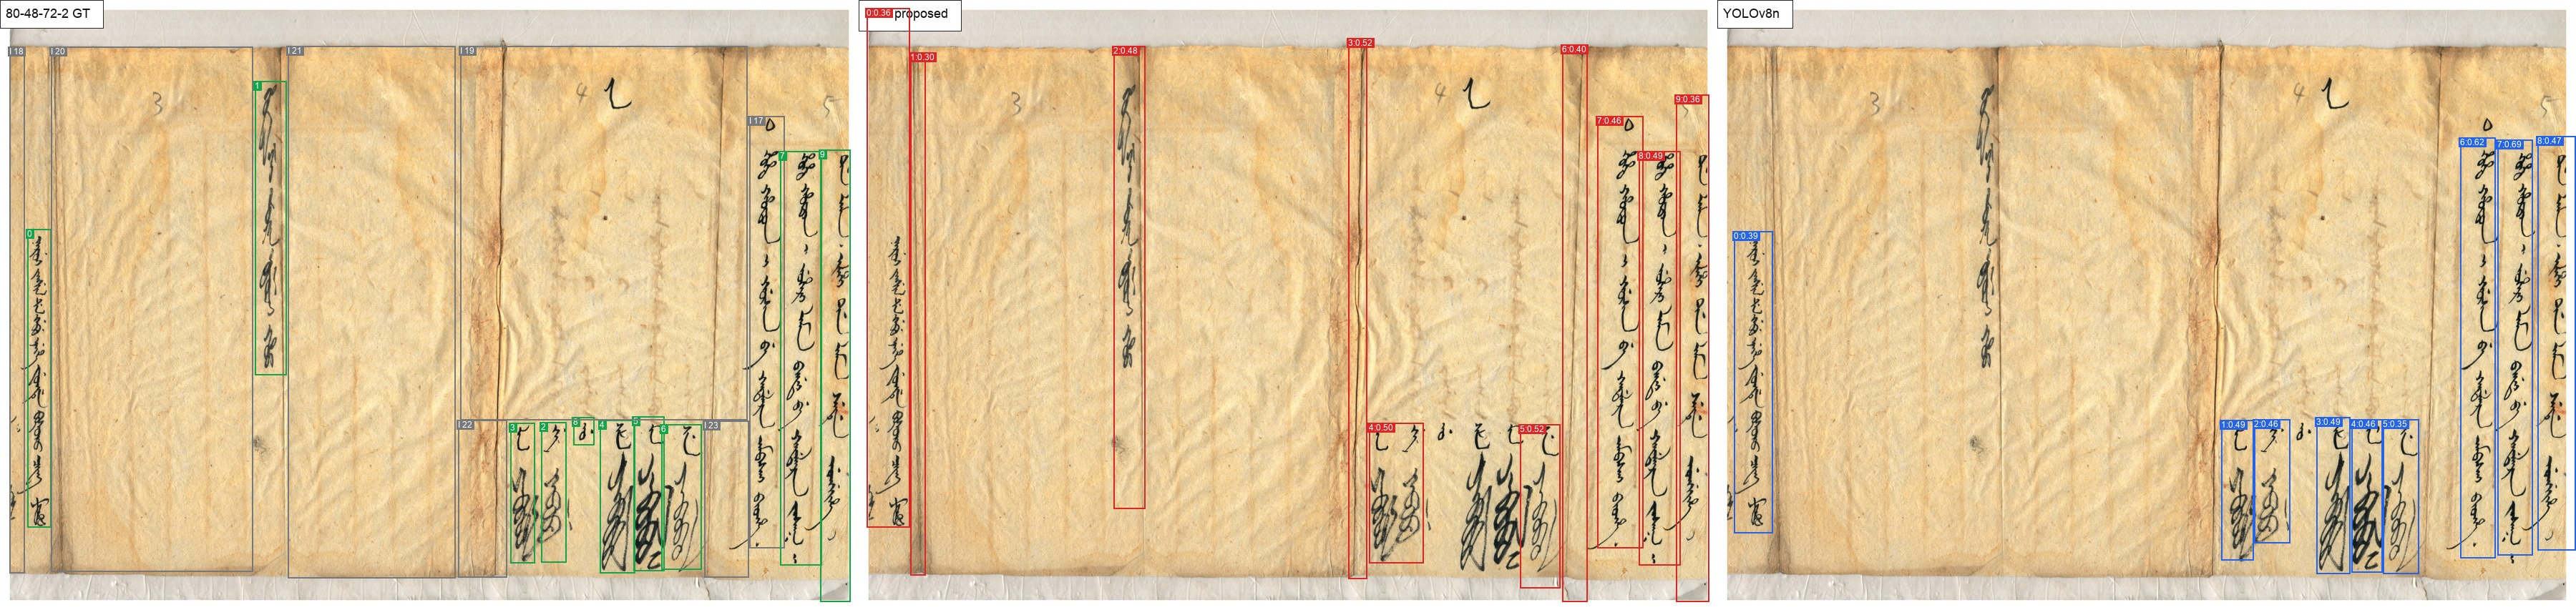
\includegraphics[width=\linewidth]{figures/page_layout_gt_rule_yolo.jpg}
    \caption{Qualitative page-level column detection comparison. Left: human GT annotations; middle: rule-based proposed detector; right: YOLOv8n with rotation-aware reading-order recovery. Green, red, and blue boxes denote GT, rule-based predictions, and YOLO predictions, respectively.}
    \label{fig:page_layout_comparison}
\end{figure}


\begin{table}[htbp]
\centering
\caption{Confidence-threshold sensitivity of YOLOv8n. The final threshold is selected on the validation split rather than on the test split.}
\label{tab:yolo_threshold_sensitivity}
\begin{tabular}{l c c c c}
\toprule
\textbf{Split} & \textbf{Threshold} & \textbf{Prec.} & \textbf{Rec.} & \textbf{F1} \\
\midrule
Validation & 0.25 & 0.746 & 0.787 & 0.766 \\
Validation & 0.30 & 0.812 & 0.759 & 0.785 \\
Validation & 0.35 & \textbf{0.876} & 0.722 & \textbf{0.792} \\
\midrule
Test & 0.25 & 0.858 & 0.779 & 0.817 \\
Test & 0.30 & 0.894 & 0.675 & 0.769 \\
Test & 0.35 & \textbf{0.919} & 0.626 & 0.745 \\
\bottomrule
\end{tabular}
\end{table}

The threshold sensitivity in Table~\ref{tab:yolo_threshold_sensitivity} suggests that the detector is robustly stronger than the rule-based baseline across a practical threshold range, but the precision--recall trade-off remains non-negligible. In particular, a lower threshold improves recall on the test split, whereas the validation-selected threshold favors high precision.

\subsection{Ablation Studies}

\subsubsection{Complete Pipeline Ablation}
Table \ref{tab:pipeline_ablation} details the incremental contribution of each module. SASE provides the largest initial drop by mitigating the visual gap, while VS-MSSE and DANN align features effectively. Pseudo-labeling (PL) refines the conditional distribution.

\begin{table}[htbp]
\centering
\caption{Complete Pipeline Ablation (Mean $\pm$ Std).}
\label{tab:pipeline_ablation}
\begin{tabular}{l c c}
\toprule
\textbf{Configuration} & \textbf{CER (\%)} & \textbf{WER (\%)} \\
\midrule
Source Only & $34.6 \pm 1.2$ & $58.2 \pm 1.8$ \\
+ SASE & $25.1 \pm 0.9$ & $45.4 \pm 1.5$ \\
+ SASE + VS-MSSE & $19.8 \pm 0.7$ & $36.7 \pm 1.1$ \\
+ SASE + VS-MSSE + DANN & $10.4 \pm 0.3$ & $19.5 \pm 0.6$ \\
\textbf{+ Full (w/ Pseudo-Label)} & \textbf{7.8} $\pm$ \textbf{0.2} & \textbf{14.2} $\pm$ \textbf{0.4} \\
\bottomrule
\end{tabular}
\end{table}

\subsubsection{SASE Component Ablation}
Table \ref{tab:sase_ablation} isolates the contribution of individual SASE components on the Source-only model evaluated on the target test set. Ink diffusion ($D$) proves to be the most critical physical property, as its removal causes the most severe performance degradation.

\begin{table}[htbp]
\centering
\caption{SASE Component Ablation (evaluated on target test set).}
\label{tab:sase_ablation}
\begin{tabular}{l c c}
\toprule
\textbf{Configuration} & \textbf{CER (\%)} & \textbf{WER (\%)} \\
\midrule
Full SASE (Source Only) & \textbf{25.1} $\pm$ \textbf{0.9} & \textbf{45.4} $\pm$ \textbf{1.5} \\
\midrule
w/o structural jitter ($\sigma$) & $27.2 \pm 1.0$ & $48.1 \pm 1.6$ \\
w/o ink diffusion ($D$) & $29.6 \pm 1.1$ & $52.3 \pm 1.7$ \\
w/o archival background patches & $28.1 \pm 0.9$ & $50.0 \pm 1.5$ \\
\bottomrule
\end{tabular}
\end{table}

\subsubsection{VS-MSSE Architectural Ablation}
Table \ref{tab:msse_ablation} justifies the asymmetrical design. Compared to symmetrical ASPP ($3\times3$), VS-MSSE ($5\times1$) achieves superior performance with fewer FLOPs by eliminating unnecessary horizontal computation paths. Expanding to $7\times1$ provides diminishing returns and increases parameter count. 

\begin{table}[htbp]
\centering
\caption{VS-MSSE Configuration Ablation (evaluated at +DANN stage).}
\label{tab:msse_ablation}
\begin{tabular}{l c c c}
\toprule
\textbf{Module Architecture} & \textbf{Params (M)} & \textbf{FLOPs (G)} & \textbf{CER (\%)} \\
\midrule
Standard ResNet-34 & 21.3 & 3.6 & $14.1 \pm 0.5$ \\
Symmetrical ASPP ($3\times3$) & 24.5 & 4.2 & $12.5 \pm 0.4$ \\
VS-MSSE (Kernel $3\times1$) & 22.8 & 3.8 & $11.6 \pm 0.3$ \\
\textbf{VS-MSSE (Kernel $5\times1$)} & 23.4 & 3.9 & \textbf{10.4} $\pm$ \textbf{0.3} \\
VS-MSSE (Kernel $7\times1$) & 24.1 & 4.1 & $10.3 \pm 0.3$ \\
\bottomrule
\end{tabular}
\end{table}

\section{Error Analysis and Limitations}
Grad-CAM visualizations confirm that VS-MSSE highly activates along the central vertical spine. A quantitative breakdown of the remaining errors ($7.8\%$ CER)—computed over manually categorized character-level errors on the test set—reveals three primary failure modes:
\begin{itemize}[noitemsep,topsep=0pt]
    \item \textbf{Deletion due to broken spines (42\%):} Extreme physical trauma (e.g., severe water damage or paper folding) dissolves the vertical axis, causing the CTC decoder to skip characters.
    \item \textbf{Substitution among visually similar vowels (35\%):} In 19th-century cursive, scribes routinely abbreviated trailing vowels (e.g., `A` vs. `E`), creating profound topological ambiguity.
    \item \textbf{Insertion caused by stains/noise (23\%):} Dark oxidative stains intersecting the spine are occasionally hallucinated as consonants.
\end{itemize}
The main recognition framework still assumes isolated text lines, and the page-level detector is currently evaluated as a pilot upstream extension rather than a fully integrated end-to-end OCR system. Although the YOLOv8n detector substantially improves page-level column extraction, confidence-threshold sensitivity and rare failures on pages with very few columns remain limitations. Future work will integrate page detection, reading-order recovery, and the UDA recognizer into a single end-to-end archival OCR pipeline, especially for full folios containing complex layout noise such as imperial red seals stamped directly over textual columns.

\section{Data Availability and Reproducibility Statement}
An anonymized repository containing training scripts, configuration files, random seeds, synthetic generator parameters, model checkpoints, and the evaluation protocol will be provided as supplementary material during the review process. While the authentic archival dataset is subject to institutional copyright, a desensitized subset of strictly isolated column patches (with no sensitive metadata) will be included in the repository to ensure full reproducibility.

\section{Conclusion}
This paper establishes a robust Unsupervised Domain Adaptation baseline for isolated traditional Mongolian historical text line recognition. By introducing the physical SASE engine, the geometry-aware VS-MSSE module, and correcting the CTC-entropy pseudo-label strategy, we achieved a highly statistically significant CER of $7.8 \pm 0.2\%$, providing a key recognition component for future large-scale digital humanities pipelines for low-resource vertical scripts. In addition, our pilot page-level column detection experiment demonstrates that lightweight learning-based layout analysis can substantially outperform rule-based extraction, suggesting a practical path toward full-page traditional Mongolian archival OCR.

\begin{thebibliography}{99}

\bibitem{shi2016end}
B. Shi, X. Bai, and C. Yao, ``An end-to-end trainable neural network for image-based sequence recognition,'' \textit{IEEE Transactions on Pattern Analysis and Machine Intelligence}, vol. 39, no. 11, pp. 2298--2304, 2016.

\bibitem{graves2006connectionist}
A. Graves, S. Fern{\'a}ndez, F. Gomez, and J. Schmidhuber, ``Connectionist temporal classification: labelling unsegmented sequence data with recurrent neural networks,'' in \textit{Proceedings of the 23rd international conference on Machine learning}, 2006, pp. 369--376.

\bibitem{li2021trocr}
M. Li, T. Lv, L. Cui, Y. Lu, D. Florencio, C. Zhang, Z. Li, and F. Wei, ``TrOCR: Transformer-based optical character recognition with pre-trained models,'' in \textit{Proceedings of the AAAI Conference on Artificial Intelligence}, vol. 37, no. 1, 2023, pp. 1309--1317.

\bibitem{bautista2022parseq}
D. Bautista and R. Atienza, ``Scene text recognition with permuted autoregressive sequence models,'' in \textit{European Conference on Computer Vision}, Springer, 2022, pp. 178--196.

\bibitem{ganin2015unsupervised}
Y. Ganin and V. Lempitsky, ``Unsupervised domain adaptation by backpropagation,'' in \textit{International conference on machine learning}, PMLR, 2015, pp. 1180--1189.

\bibitem{long2018conditional}
M. Long, Z. Cao, J. Wang, and M. I. Jordan, ``Conditional adversarial domain adaptation,'' \textit{Advances in neural information processing systems}, vol. 31, 2018.

\bibitem{zhu2017unpaired}
J.-Y. Zhu, T. Park, P. Isola, and A. A. Efros, ``Unpaired image-to-image translation using cycle-consistent adversarial networks,'' in \textit{Proceedings of the IEEE international conference on computer vision}, 2017, pp. 2223--2232.

\bibitem{hoffman2018cycada}
J. Hoffman, E. Tzeng, T. Park, J.-Y. Zhu, P. Isola, K. Saenko, A. Efros, and T. Darrell, ``CyCADA: Cycle-consistent adversarial domain adaptation,'' in \textit{International conference on machine learning}, PMLR, 2018, pp. 1989--1998.

\bibitem{tzeng2014deep}
E. Tzeng, J. Hoffman, N. Zhang, K. Saenko, and T. Darrell, ``Deep domain confusion: Maximizing for domain invariance,'' \textit{arXiv preprint arXiv:1412.3474}, 2014.

\bibitem{kang2020complex}
L. Kang, P. Riba, M. Rusi{\~n}ol, A. Forn{\'e}s, and M. Villegas, ``Complex document image binarization from an encoder-decoder perspective,'' \textit{Pattern Recognition}, vol. 111, p. 107663, 2021.

\bibitem{parvez2013arabic}
M. T. Parvez and S. A. Mahmoud, ``Offline Arabic handwritten text recognition: A survey,'' \textit{ACM Computing Surveys (CSUR)}, vol. 45, no. 2, pp. 1--35, 2013.

\bibitem{shi2018aster}
B. Shi, M. Yang, X. Wang, P. Lyu, C. Yao, and X. Bai, ``ASTER: An attentional scene text recognizer with flexible rectification,'' \textit{IEEE Transactions on Pattern Analysis and Machine Intelligence}, vol. 41, no. 9, pp. 2035--2048, 2018.

\bibitem{zhao2020unsupervised}
M. Zhao, Y. Li, M. M. Lu, and X. Bai, ``Unsupervised domain adaptation for scene text recognition via adversarial feature alignment and pseudo label refinement,'' \textit{Pattern Recognition}, vol. 108, p. 107559, 2020.

\bibitem{tensmeyer2017document}
C. Tensmeyer and T. Martinez, ``Document image binarization with fully convolutional neural networks,'' in \textit{2017 14th IAPR International Conference on Document Analysis and Recognition (ICDAR)}, vol. 1. IEEE, 2017, pp. 99--104.

\bibitem{zhang2019sequence}
Y. Zhang, S. Nie, W. Liu, X. Xu, D. Zhang, and H. T. Shen, ``Sequence-to-sequence domain adaptation network for robust text recognition,'' in \textit{Proceedings of the IEEE/CVF Conference on Computer Vision and Pattern Recognition}, 2019, pp. 2740--2749.

\bibitem{marti2001using}
U.-V. Marti and H. Bunke, ``Using a statistical language model to improve the performance of an HMM-based cursive handwriting recognition system,'' \textit{International Journal of Pattern Recognition and Artificial Intelligence}, vol. 15, no. 01, pp. 65--90, 2001.

\bibitem{kang2022pay}
L. Kang, P. Riba, M. Rusi{\~n}ol, A. Forn{\'e}s, and M. Villegas, ``Pay attention to what you read: Non-recurrent handwritten text recognition,'' \textit{Pattern Recognition}, vol. 129, p. 108766, 2022.

\bibitem{souibgui2022few}
M. A. Souibgui, A. Forn{\'e}s, Y. Kessentini, and C. Tudor, ``A few-shot learning approach for historical ciphered manuscript recognition,'' \textit{Pattern Recognition}, vol. 122, p. 108345, 2022.

\bibitem{bhunia2021meta}
A. K. Bhunia, S. K. Ghosh, A. Shrivastava, P. N. Chowdhury, S. S. Krig, and R. Shah, ``MetaHTR: Towards writer-adaptive handwritten text recognition,'' in \textit{Proceedings of the IEEE/CVF Conference on Computer Vision and Pattern Recognition}, 2021, pp. 11622--11631.

\bibitem{coquenet2023dan}
D. Coquenet, C. Chatelain, and T. Paquet, ``DAN: A segmentation-free document attention network for handwritten document recognition,'' \textit{IEEE Transactions on Pattern Analysis and Machine Intelligence}, vol. 45, no. 7, pp. 8227--8243, 2023.

\bibitem{fang2021read}
S. Fang, H. Xie, Y. Wang, Z. Mao, and Y. Zhang, ``Read like humans: Autonomous, bidirectional and iterative language modeling for scene text recognition,'' in \textit{Proceedings of the IEEE/CVF Conference on Computer Vision and Pattern Recognition}, 2021, pp. 7098--7107.

\bibitem{chen2021text}
X. Chen, L. Jin, Y. Zhu, C. Luo, and T. Wang, ``Text recognition in the wild: A survey,'' \textit{ACM Computing Surveys (CSUR)}, vol. 54, no. 2, pp. 1--35, 2021.

\end{thebibliography}

\end{document}
